\documentclass{article}
\usepackage{tikz}

\begin{document}

%! \usetikzlibrary{decorations.pathreplacing,decorations.pathmorphing}
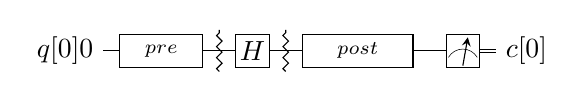
\begin{tikzpicture}[scale=1.000000,x=1pt,y=1pt]
\filldraw[color=white] (0.000000, -7.500000) rectangle (142.000000, 7.500000);
% Drawing wires
% Line 2: q0 W q[0]\ket{0} c[0]
\draw[color=black] (0.000000,0.000000) -- (130.000000,0.000000);
\draw[color=black] (130.000000,-0.500000) -- (142.000000,-0.500000);
\draw[color=black] (130.000000,0.500000) -- (142.000000,0.500000);
\draw[color=black] (0.000000,0.000000) node[left] {$q[0]\ket{0}$};
% Done with wires; drawing gates
% Line 3: q0 G:width=30 $pre$
\begin{scope}
\draw[fill=white] (21.000000, -0.000000) +(-45.000000:21.213203pt and 8.485281pt) -- +(45.000000:21.213203pt and 8.485281pt) -- +(135.000000:21.213203pt and 8.485281pt) -- +(225.000000:21.213203pt and 8.485281pt) -- cycle;
\clip (21.000000, -0.000000) +(-45.000000:21.213203pt and 8.485281pt) -- +(45.000000:21.213203pt and 8.485281pt) -- +(135.000000:21.213203pt and 8.485281pt) -- +(225.000000:21.213203pt and 8.485281pt) -- cycle;
\draw (21.000000, -0.000000) node {\scriptsize$pre$};
\end{scope}
% Line 4: BARRIER
\draw[decorate,decoration={zigzag,amplitude=1pt,segment length=4}] (42.000000,-7.500000) -- (42.000000,7.500000);
% Line 5: q0 H
\begin{scope}
\draw[fill=white] (54.000000, -0.000000) +(-45.000000:8.485281pt and 8.485281pt) -- +(45.000000:8.485281pt and 8.485281pt) -- +(135.000000:8.485281pt and 8.485281pt) -- +(225.000000:8.485281pt and 8.485281pt) -- cycle;
\clip (54.000000, -0.000000) +(-45.000000:8.485281pt and 8.485281pt) -- +(45.000000:8.485281pt and 8.485281pt) -- +(135.000000:8.485281pt and 8.485281pt) -- +(225.000000:8.485281pt and 8.485281pt) -- cycle;
\draw (54.000000, -0.000000) node {$H$};
\end{scope}
% Line 6: BARRIER
\draw[decorate,decoration={zigzag,amplitude=1pt,segment length=4}] (66.000000,-7.500000) -- (66.000000,7.500000);
% Line 7: q0 G:width=40 $post$
\begin{scope}
\draw[fill=white] (92.000000, -0.000000) +(-45.000000:28.284271pt and 8.485281pt) -- +(45.000000:28.284271pt and 8.485281pt) -- +(135.000000:28.284271pt and 8.485281pt) -- +(225.000000:28.284271pt and 8.485281pt) -- cycle;
\clip (92.000000, -0.000000) +(-45.000000:28.284271pt and 8.485281pt) -- +(45.000000:28.284271pt and 8.485281pt) -- +(135.000000:28.284271pt and 8.485281pt) -- +(225.000000:28.284271pt and 8.485281pt) -- cycle;
\draw (92.000000, -0.000000) node {\scriptsize$post$};
\end{scope}
% Line 8: q0 M
\draw[fill=white] (124.000000, -6.000000) rectangle (136.000000, 6.000000);
\draw[very thin] (130.000000, 0.600000) arc (90:150:6.000000pt);
\draw[very thin] (130.000000, 0.600000) arc (90:30:6.000000pt);
\draw[->,>=stealth] (130.000000, -5.400000) -- +(80:10.392305pt);
% Done with gates; drawing ending labels
\draw[color=black] (142.000000,0.000000) node[right] {$c[0]$};
% Done with ending labels; drawing cut lines and comments
% Done with comments
\end{tikzpicture}
\end{document}
